\documentclass[paper=a4paper,fontsize=10pt]{jlreq}
% パッケージの読み込み
\usepackage{luatexja-fontspec}
\usepackage{graphicx}
\setmainfont{Harano Aji Mincho}
\setsansfont{Harano Aji Gothic}
\setmainjfont{Harano Aji Mincho}
\setsansjfont{Harano Aji Gothic}

\usepackage{amsmath,amssymb}
\usepackage{unicode-math}
\setmathfont{LatinModernMath-Regular}

\graphicspath{{img/}}

\title{\huge 令和6年度 修士論文\\\vspace{100truept}プログラム読解における\\視線運動のクラスタリング\\
Clustering of Eye Movements\\ in Program Reading}
\author{\large 大阪公立大学大学院 \\情報学研究科 基幹情報学専攻\\学籍番号 BGA23116\\明石 拓也}


\begin{document}
\maketitle
\clearpage

\tableofcontents
\clearpage

\part{はじめに}
  \section{研究背景}
  情報活用能力が必要となった近年において、初等教育からプログラミングが必修化されるなどプログラミング教育の機会は増加している。一方で、プログラミングに長けた指導者の不足が問題視されている。そのため、プログラミング学習の支援となるシステムの重要性が高まっている。学習システム開発のためには、プログラミングを理解している人の読解方法の傾向をつかむことが重要となっている。
  プログラミング学習支援において、プログラム読解過程の分析、特にプログラミングを理解しているかに応じた分析は、プログラミング学習者の支援において有用であることが示されている。
    

  \section{研究目的}


\part{関連研究}


\part{提案手法}


\part{実験}
  本章では、実験に際し行った準備と、実験の手順を示す。
  
  本章の大まかな流れを以下に示す。
  \begin{enumerate}
    \item 実験準備
      \begin{enumerate}
        \item iTrace-Atomプラグインの開発
        \item 各PCの環境構築
      \end{enumerate}
    \item 実験
      \begin{enumerate}
        \item 被験者入場
        \item 解答用紙への氏名記入・同意書記入
        \item キャリブレーション
        \item 実験の流れの説明
        \item 練習問題
        \item 5つのタスク
        \item 被験者退場
      \end{enumerate}
  \end{enumerate}

  \section{実験準備}
    実験に際して、

  \section{実験}

    \begin{figure}[htbp]
      \centering
      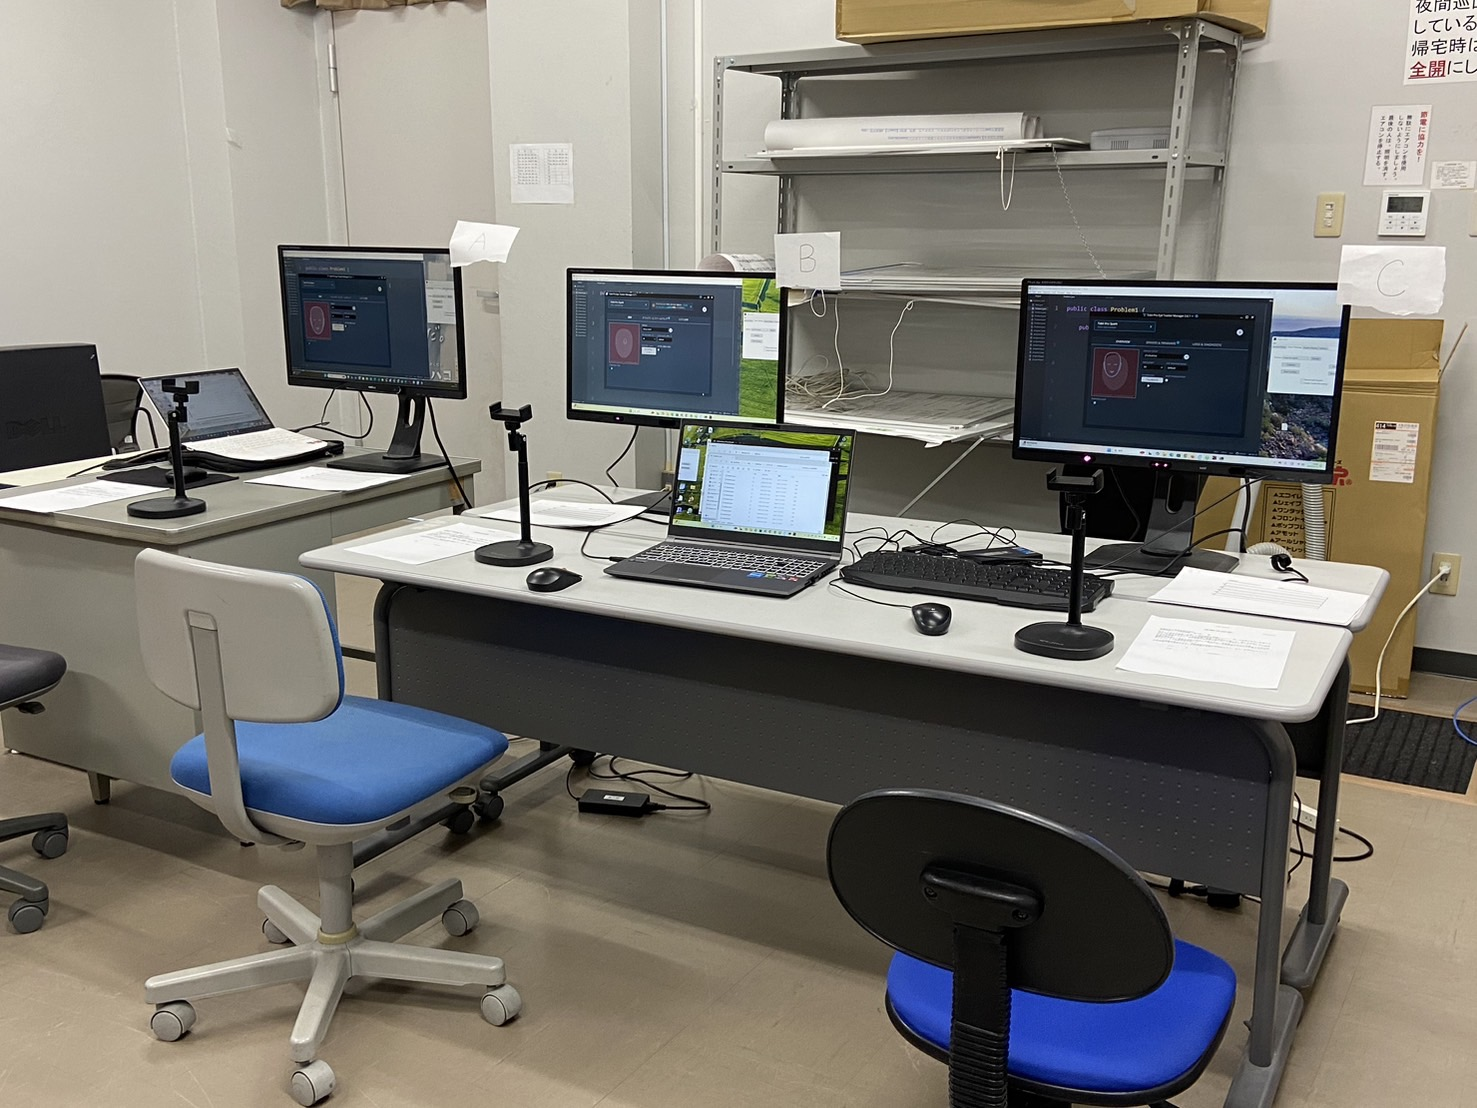
\includegraphics[width=0.8\linewidth]{実験部屋.jpg}
      \caption{実験部屋の様子}
    \end{figure}

\part{データの分析}


\part{結論}


\begin{thebibliography}{99}
  \bibitem{uwano} 構文木と視線移動の自動マッピング手法を用いたプログラム理解過程の分析,吉岡春彦,上野秀剛,2023
  \bibitem{tobii} tobii pro spark https://www.tobii.com/ja/products/eye-trackers/screen-based/tobii-pro-spark
  \bibitem{itrace} iTrace https://www.i-trace.org/
  \bibitem{atom} ATOM https://atom-editor.cc/
\end{thebibliography}


\end{document}
